\documentclass{article}

\usepackage{mathtools}
\DeclarePairedDelimiter\ceil{\lceil}{\rceil}
\DeclarePairedDelimiter\floor{\lfloor}{\rfloor}


\usepackage{graphicx}

\begin{document}

\title{Evolving Random Graph Generating Algorithms}

\author{
Pope, Aaron\\
\texttt{aaron.pope@mst.edu}
\and
Martin, Matthew\\
\texttt{mam446@mst.edu}
}

\maketitle

\section{Introduction}

\subsection{Random Graphs}

Random graphs have a variety of applications in graph theory. The graphs themselves can be described as a model consisting of a probability distribution of degrees, adjacency or some other characteristic. Alternatively, random graphs can be described by a stochastic process of generating a graph within certain constraints. The research presented in this work will focus on this latter approach.

How well a random graph model describes a given graph can be determined by performing a statistical goodness of fit test. Inversely, if a random process is to produce graphs which fit well with a given random graph model, a goodness of fit test performed on a population of resulting graphs with respect to the desired model can be used to determine how well the process produces graphs described by the model. 

It is possible to have desirable features within a graph that are not captured or guaranteed by a random graph model. An example of this would be the occurrence of certain topology motifs within the graph. The presence of these motifs can have a large impact on characteristics of the graph as a whole, such as the resilience or robustness of the graph. These motifs, along with other features, can be detected in the graphs which are generated by a given process. The quality of the graph generating process can be determined by how consistently it produces graphs with a high occurrence of desirable features and a low occurrence of undesirable features.

\subsection{Evolutionary Computing and Genetic Programming}

Evolutionary Computing (EC) uses a biologically inspired process to solve a problem by generating a population of potential solutions and selecting the best among them to participate in procreation to create more solutions. This process continues through multiple generations until certain termination criteria are met. Genetic Programming (GP) is a field of EC in which the solutions sought are programs themselves. The candidate programs can be represented as parse trees in which the internal nodes represent operations on the input received from the children nodes and the leaf nodes are chosen from the problem's input.

Traditional GP has several stochastic components. The population is initialized with randomly created solutions, offspring inherit a random selection of attributes from each parent and each offspring has a chance of undergoing a random mutation. Because of these stochastic elements, a GP algorithm will explore possible solutions that might seem counterintuitive to a human developer. While these non-obvious choices are usually inferior, they can, on occasion, lead to a breakthrough in computational efficiency or solution accuracy.

A major challenge in implementing a GP algorithm is creating a set of operations which can be combined to create a candidate solution. The operation set needs to contain a variety of methods in order for the GP to create solutions to a variety of problem types. However, if the set grows too large, the search space of potential solutions explodes, making a search infeasible. Therefore, the goal is to find a minimal set of operations which are crucial to solving a specific problem or family of problems.

Another challenge is measuring the quality of a candidate solution when determining which solutions will survive and procreate. In EC, this measure is known as the fitness of the solution. Often the process of evaluating the fitness of individual solutions in the population is the performance bottleneck of the evolutionary algorithm. For this reason, it is desirable to have an efficient method of evaluating a solution's quality. Even if no such efficient evaluation method is available, using genetic programming can still be beneficial. If the GP algorithm seeks to replace a program which is more efficient than another which is commonly used, then the time to find a new highly specialized solution can be justified.

If an optimal fitness value is known, potential solutions can be compared to this ideal value to determine their quality. If an optimal solution value is not known, the individuals in the population can be compared to one another to determine relative quality. To evaluate the quality of a GP solution, the parse tree representation is converted to a program which is run with a set of various input samples. The accuracy of the program's output is used to measure the quality of the solution.

The method of evaluating random graph generating programs will depend on the type of problem the GP used to solve. If a program is sought which produces graphs that adhere to a specific random graph model, then the program can be used to generate a set of graphs which are evaluated using a goodness of fit test to determine how well they fit the desired model. If the goal is instead to generate graphs which exhibit some feature, the program can be evaluated by determining the rate of occurrence of these features in the graphs it produces. Programs produce graphs that adhere better to the intended model or have a higher rate of occurrence for desirable features will have higher relative fitness values.

\section{Related Work}

Random graphs and random graph models have been studied extensively in various applications
in previous research. Some simple models use independent probabilities for the presence of
each edge~\cite{Erdos:59,Erdos:60}. Exponential random graph models use vertex degree
distributions which have been found to resemble the structure of social and other types of
networks~\cite{Wasserman:94,Robins:07}. Wireless sensor networks have been modeled as random
geometric graphs which are created by placing vertices randomly within an area and connecting
vertices within a certain radius of each other~\cite{Avin:07,Diaz:01}.
 
There have been many works done on evolving algorithms to do a specific 
task~\cite{Lourenco:12,Martin:13}. However, there have been no applications of evolving
random graph generating algorithms or graph algorithms in general. Though the application of 
the work in evolving algorithms is different from the goals of this paper, the concepts that
those algorithms are based on can be used in this application. These papers use Koza style 
GP~\cite{Koza:92} and Grammatical Evolution~\cite{Ryan:98}. In this paper, Koza
style GP will be used to construct the random graph generating algorithm. 

\section{Motivation}

The goal of this research is to develop a general purpose genetic algorithm which evolves programs that generate random graphs that satisfy certain constraints. This would provide a source of material that could be used to facilitate further research in various areas of graph theory. For instance, if researchers want to examine the efficiency of a new networking algorithm when applied to scale free networks, a program which generates power law distribution graphs can be evolved and used to generate test graphs. The versatility of the genetic algorithm approach will allow this to be done even when the desired features of a random graph are difficult to express within a random graph model.

\section{Methodology}

\begin{figure}
\begin{centering}
  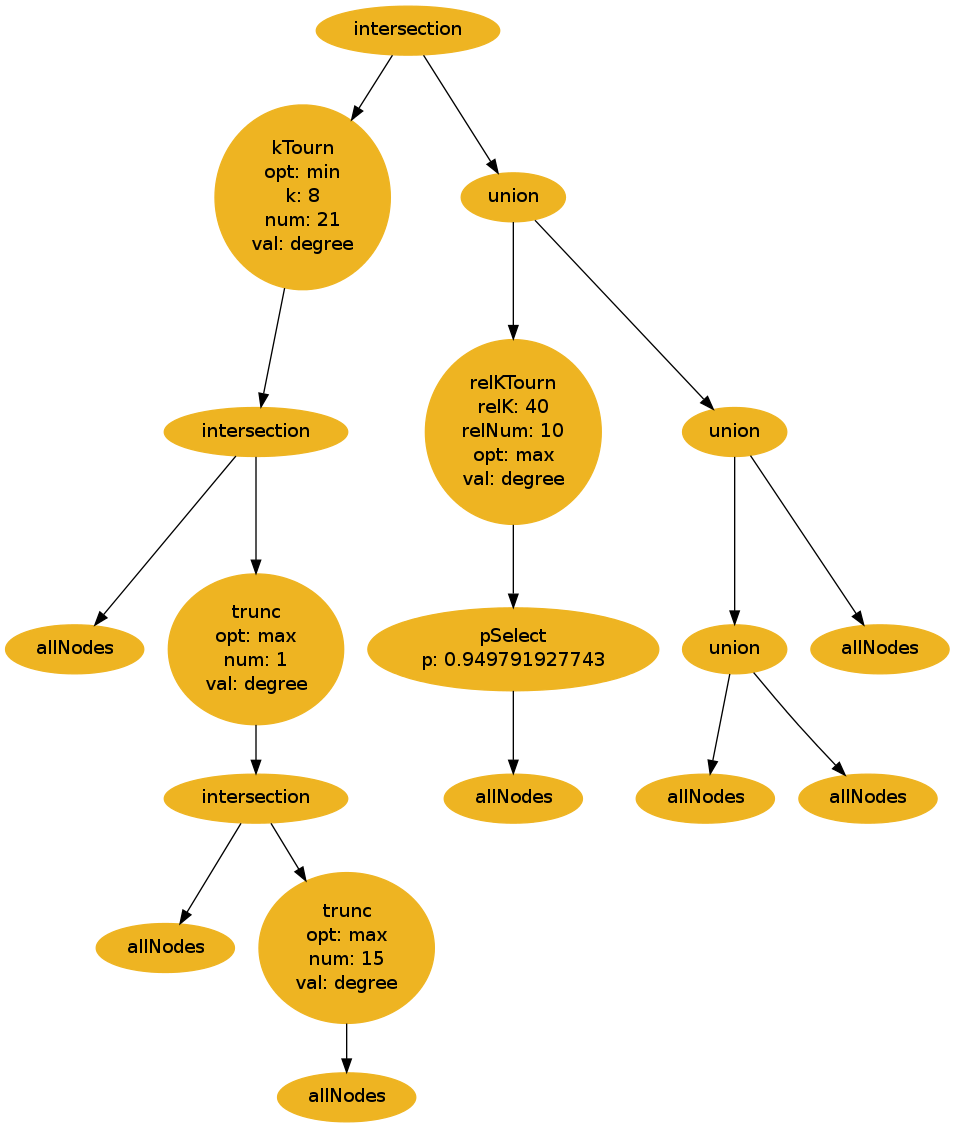
\includegraphics[scale=0.4]{RandomGraphExample2.png}
  \caption{Example Random Graph Generating Parse Tree}
  \label{fig:example}
\end{centering}
\end{figure}


This paper discusses a method using GP to evolve an algorithm that generates a random graph 
of with a specified nature.  The method proposed uses Koza style GP to evolve a post-ordered 
parse tree structure that will represent the algorithm. Most random-graph generating algorithms 
repeat a node adding phase $n$ times to create a random graph of size $n$. Our algorithm takes 
advantage of this repetitive nature of random-graph algorithms in such a way that it only 
evolves the method for adding a vertex and its connections. In this phase, the parse tree decides 
which vertices will be adjacent to the new vertex.


\subsection{Parse-Tree}
There are two proposed methods that this decision process can be done. One method is for each new vertex, 
the algorithm would iterate over every existing vertex and the parse tree would determine if a 
connection would be made between that vertex and the new vertex. The second method would be for the parse 
tree to be evaluated one time and determine the set of vertices to which the new node will be connected.  
It was determined that the second method would be the preferred option, as it would be easier to 
construct some of the pre-existing random graph algorithms such as the Erd\H{o}s-R\'{e}nyi model.

\subsection{Nodes}
The parse tree will be constructed from a set of operations that will be used as the non-terminal 
nodes. Sets of vertices which will be used as the terminal nodes in the parse tree.  Each of the operations will take 
in one or more sets of vertices and return a single set of vertices. The set of vertices returned by the 
root node will be the set of vertices that the newly created vertex will connect to. 
An example parse tree can be seen in Figure \ref{fig:example}.

There are two primary types of non-terminal operations that are used as nodes in the construction of the parse-tree. The
first of which are selection operations. These operations take a set of vertices and by some method selects vertices from
that set and returns them to its parent node. The second type of non-terminal operations are set operations. These nodes 
typically take two sets of vertices and perform some kind of set operation on the two sets and return the product to its
parent node. The exact specifications of the operations that were used as nodes can be found below.

\subsubsection{Selection Nodes}
There are two types of selection nodes that were used to evolve the Random Graph Algorithms. The first of which are standard
selection operations that have constant values for their parameters. The second are relative selection operations. For this 
second type of selection operations, the parameter values used are relative to the size of the graph. This addition was made
so that the Random Graph Algorithms would create graphs with the same properties as the size of the graph increased substantially. 

In a majority of the selection operations, the vertices are compared to one another to determine selection. When this is the case, 
they are compared based upon some measure of the node. In the experiments reported in this paper, the only measure that was available
was the degree of the vertex. This however could be any measure of a node such as its eccentricity or other measures. For these
selection operations that are based on vertex measures, the selection can be done as a minimization or maximization of that measure. For
example, the operation could try to select vertices with a high degree or select vertices with a low degree.

For the first type of selection operation, there were four selection operations that were used. The first of which is call `p-Select'.
This selection operation iterates over the set of vertices that were passed in and has a $p$ probability of selecting each vertex. The
second selection operation is the standard k-Tournament selection with replacement. This operation has two parameters; one of which is $k$ which
is the number of vertices to compare each iteration, and $num$ which is the number of vertices selected and passed to its parent node. Note that 
vertices can be reselected during the selection process, they will not appear multiple times in the sets that are passed to its parent. This 
is done to insure that the resulting random graphs are simple. The third selection operation is a random sub-set operation. This operation takes 
a random sub-set of size $n$ from the set passed and returns that set to its parent node. This selection is done without replacement. The fourth 
selection operation is truncation selection. This operation selects the highest or lowest $n$ vertices based on the measure specified, and passes
them to its parent node.

The second type of selection operation is relative selections. There are three selection operations of this type used in the experiments presented
in this paper. They are the k-Tournament selection, random sub-set selection and truncation selection that were presented earlier. The difference
in this version of the selection is that each of the parameters of the selection are relative to the size of the graph. An example of the
relation for k-Tournament's $k$ can be seen in Equation~\ref{eq:example}.

\begin{equation}
\label{eq:example}
k_{val} = \floor*{\frac{n}{k_{rel}}}
\end{equation}

In the above equation, $k_{val}$ is the $k$ value that is used for that run of the k-Tournament function, $n$ is the number of vertices in the graph, and $k_{rel}$
is a constant parameter value that is associated with that k-Tournament node.


\subsubsection{Set Nodes}

The second type of operation that is used in the presented experiments are set operations. All of these operations take two sets of vertices and return
a single set of vertices to its parent node. There are four set operations that are used in the experiments. The first is the union operation which returns
the vertices which are in both sets passed in. The second is the intersection which returns the vertices which are in common between the two sets passed in. 
The third is the difference operation which returns the vertices that are in the left child's set but not in the right child's. The fourth is the symmetric
difference operation which returns the vertices that are in either the left child's set or the right child's set but not in both. 


\subsection{Genetic Program}
GP is employed to meta-evolve the Random Graph Algorithms. The two primary variation operators employed are the standard sub-tree crossover and the sub-tree
mutation operator altered to make the maximum number of nodes being added a user defined value. Another mutation operation was added to this algorithm that 
selects a node at random from the parse tree and randomizes the parameters if it has any; if the node does not have any parameters the mutation is executed again. 
The parameters are set to a random valued within a specified user range for each nodes parameters. This can also alter the type of measure used in the selection
operations and if the selections attempt to minimize or maximize the measure. 

\subsubsection{Random Graph Algorithm}
Each individual in the GP population encodes a Random Graph Algorithm. To evaluate the fitness of an individual its encoded Random Graph Algorithm generates
a random graph a user-defined number of times. The resulting graphs are generated to be the same size to ensure an accurate fitness. These graphs are evaluated 
using a user defined fitness function. The fitness of the Random Graph Algorithm is the average fitness of the graphs that it produces. 

The graphs are generated by iteratively executing the parse-tree. Each iteration a single vertex is added to the graph and the parse tree is executed to determine
which vertices the new vertex will share an edge with. By employing this method, every possible graph is possible to be generated assuming that the right operations 
are available for the evolution process. 

\subsubsection{Fitness Calculation}
For the experiments presented in this paper, there were many different fitness functions employed to demonstrate the capabilities of the algorithm that
is proposed. The primary graph characteristics that were employed for fitness functions were graph partitioning, eccentricity, and the number of edges.  
Four fitness functions were constructed from these graph characteristics and using during evolution. For each of the functions, it was required that the graph
be connected. If the graph was not connected the fitness value was set to an arbitrarily small value.

The first fitness function was designed to maximize 
the edgecut needed to partition the graph into two pieces while minimizing the number of edges in the graph. To approximate the edgecut of the partition,
the Metis algorithm was used. The edges are minimized to prevent a complete graph from being always evolved. This fitness function can be seen in Equation~\ref{eq:maxMetis}.

\begin{equation}
\label{eq:maxMetis}
fitness = c_1E_c - c_2E
\end{equation}

In the above equation, $c_1$ and $c_2$ are positive weighting constants, $E_c$ is the edge cut of the graph, and $E$ is the number of edges in the graph.


The second fitness function was designed to minimize 
the edgecut needed to partition the graph into two pieces while maximizing the number of edges in the graph. To approximate the edgecut of the partition,
the Metis algorithm was used. The edges are maximized to prevent an empty graph from always being evolved. This fitness function can be seen in Equation~\ref{eq:minMetis}.

\begin{equation}
\label{eq:minMetis}
fitness = -c_1E_c + c_2E
\end{equation}

In the above equation, $c_1$ and $c_2$ are positive weighting constants, $E_c$ is the edge cut of the graph, and $E$ is the number of edges in the graph.



The third fitness function was designed to maximize the average eccentricity of a graph while trying to minimize the number of edges. The edges are minimized
to prevent a complete graph from always being evolved. This fitness function can be seen in in Equation~\ref{eq:maxEccen}.


\begin{equation}
\label{eq:maxEccen}
fitness = c_1\frac{\sum\limits_{e \in G}\epsilon_{G}(e)}{n} - c_2E
\end{equation}

In the above equation, $c_1$ and $c_2$ are positive weighting constants, $\epsilon_{G}(e)$ is the eccentricity of edge $e$, and $E$ is the number of edges in the graph.


The fourth fitness function was designed to minimize the average eccentricity of a graph while trying to minimize the number of edges. The edges are minimized to 
prevent a complete graph from always being evolved. This fitness function
can be seen in in Equation~\ref{eq:minEccen}.


\begin{equation}
\label{eq:minEccen}
fitness = -c_1\frac{\sum\limits_{e \in G}\epsilon_{G}(e)}{n} - c_2E
\end{equation}

In the above equation, $c_1$ and $c_2$ are positive weighting constants, $\epsilon_{G}(e)$ is the eccentricity of edge $e$, and $E$ is the number of edges in the graph.

For each of the fitness function parsimony pressure is added to temper the growth of the parse trees. The parsimony pressure is calculated by multiplying the number
of nodes in a tree by a user defined value. The parsimony pressure is subtracted from fitness calculated by the fitness functions defined.

\subsubsection{External Verification}
To assure that the performance of the evolved Random Graph Algorithms are consistent with their performance reported during evolution,
executable code is generated to represent the parse tree. This is done to externally verify that the performance that the GP shows for a
given Random Graph Algorithm is accurate when actually implemented. The generated code is used in all of the experiments to ensure unbiased execution 
of the Random Graph Algorithms.


\section{Experimental Setup}
The goal of this paper was to demonstrate that custom Random Graph Algorithms can be generated using GP. To demonstrate this, Random Graph Algorithms were evolved
using the four fitness functions described earlier. We then compare the evolved Random Graph Algorithms to pre-existing algorithms to demonstrate the need for new
Random Graph Algorithms for a user-defined application. Four experiments were conducted to demonstrate that a custom Random Graph Algorithm can be generated to 
create random graphs that have qualities defined by the fitness function used. Each of the experiments are conducted five times to demonstrate the ability to 
consistently evolve high-quality Random Graph Algorithms.

\begin{table}
    \begin{center}
    \begin{tabular}{|c|c|}
        \hline
        \textbf{Parameter} &\textbf{Value}\\ \hline
        Evaluations&5000\\ \hline
        Initial Population&100\\ \hline
        Children per Generation&50\\ \hline
        k-Tournament for Parent Selection&8\\ \hline
        k-Tournament for Survival Selection&5\\ \hline
	    Sub-Tree Crossover Probability& 35\% \\ \hline
	    Sub-Tree Mutation Probability& 35\% \\ \hline
	    Alternate Mutation Probability& 30\% \\ \hline
	    Alternate Mutation Depth& 5\\ \hline
	    Parsimony Pressure & 1\\ \hline
        Random Graph Algorithm Runs&20\\ \hline
        Graph Size&300\\ \hline
    \end{tabular}
    \end{center}
\caption{GP Configurations}
  \label{tab:GP}
\end{table}

Each of the four experiments will be run using the same parameter settings for the GP algorithm.  
The GP was run for 5000 evaluations. The initial population
was 100 individuals and each generation 50 new individuals were created. $k$-tournament selection with replacement 
and $k=8$ was employed for parent selection. $k$-tournament selection without replacement and $k=5$ was employed for survival selection.
The sub-tree crossover and mutation operations had 35\% chance of being used
while the alternate mutation had a probability of 30\%. The parsimony pressure for the tree size was 1.
Each Random Graph Algorithm was run 20 times during the evolution and generated graphs of size 300. 
Due to the high computational cost of running the GP, only minimal tuning was feasible. A summary
of the parameter settings for the GP can be seen in Table~\ref{tab:GP}. A summary of the constant weights used
in the fitness functions for the experiments can be seen in Table~\ref{tab:fitness}.


\begin{table}
    \begin{center}
    \begin{tabular}{|c|c|c|}
    \hline
    \textbf{Fitness Function} & \textbf{$c_1$} & \textbf{$c_2$} \\ \hline
    Maximize Edgecut&1 & 2\\ \hline
    Minimize Edgecut&50& 1 \\ \hline
    Maximize Average Eccentricity& 50 &1\\ \hline
    Minimize Average Eccentricity& 50 &1\\ \hline
    \end{tabular}
    \end{center}
    \caption{Constant weight settings for fitness functions}
    \label{tab:fitness}
\end{table}

\begin{table}
    \begin{center}
    

    \begin{tabular}{|c|c|c|}
        \hline
        \textbf{Operation} &\textbf{Parameter}&\textbf{Range/Options}\\ \hline
        p-Select & $p$ & (0,1.0)\\ \hline \hline
        k-Tournament Selection & $k$ & (1,50) \\ \hline
        * & $num$ & (1,50)\\ \hline
        * & Measure & degree \\ \hline
        * & Optimization & minimize, maximize \\ \hline \hline
        Random Subset Selection & $num$ & (1,50) \\ \hline \hline
        Truncation Selection & $num$ & (1,50) \\ \hline
        * & Measure & degree \\ \hline
        * & Optimization & minimize, maximize \\ \hline \hline

        Relative k-Tournament Selection & $k_{rel}$ & (1,50) \\ \hline
        * & $num_{rel}$ & (1,50)\\ \hline
        * & Measure & degree \\ \hline
        * & Optimization & minimize, maximize \\ \hline \hline
        Relative Random Subset Selection & $num_{rel}$ & (1,50) \\ \hline \hline
        Relative Truncation Selection & $num_{rel}$ & (1,50) \\ \hline
        * & Measure & degree \\ \hline
        * & Optimization & minimize, maximize \\ \hline

    \end{tabular}
    \end{center}
\caption{Operation Parameter Ranges}
    \label{tab:op}
\end{table}

Each operation that can be used during the evolution of the Random Graph Algorithms has parameters with user-defined ranges. For the `p-select' operation
the range that its parameter can take is from 0.0 to 1.0. For all other parameters that the other operations use, the range is from 1 to 50 inclusively.
A summary of the parameter ranges can be seen in Table~\ref{tab:op}.

\section{Results}

In all of the experiments, the Random Graph Algorithms all appeared to be very similar in structure. Also, the graphs they produced were very similar if not
identical. Figures~\ref{fig:maxM},~\ref{fig:minM},~\ref{fig:maxE}, and~\ref{fig:minE} show the parse tree representations of the typical Random Graph Algorithm
for experiments one through four respectively. Figures~\ref{fig:starGraph},~\ref{fig:minMGraph}, and~\ref{fig:minEGraph} show the typical graph generated by the
Random Graph Algorithms in experiments one, two, and four. The graphs generated by the Random Graph Algorithms in experiment were all paths and were too large to be included 
in this paper. Figures~\ref{fig:maxM-graph},~\ref{fig:minM-graph},~\ref{fig:maxE-graph}, and~\ref{fig:minE-graph} are graphs that demonstrate how the primary property of
each experiment scale as the number of vertices are scaled.


\begin{figure}
\begin{centering}
  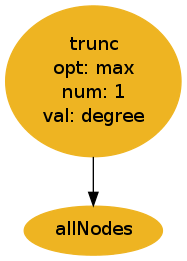
\includegraphics[scale=0.4]{maxM.png}
  \caption{Parse Tree of Random Graph Algorithm Found to Maximize the Edgecuts of a Partition and Minimize the Number of Edges}
  \label{fig:maxM}
\end{centering}
\end{figure}

\begin{figure}
\begin{centering}
  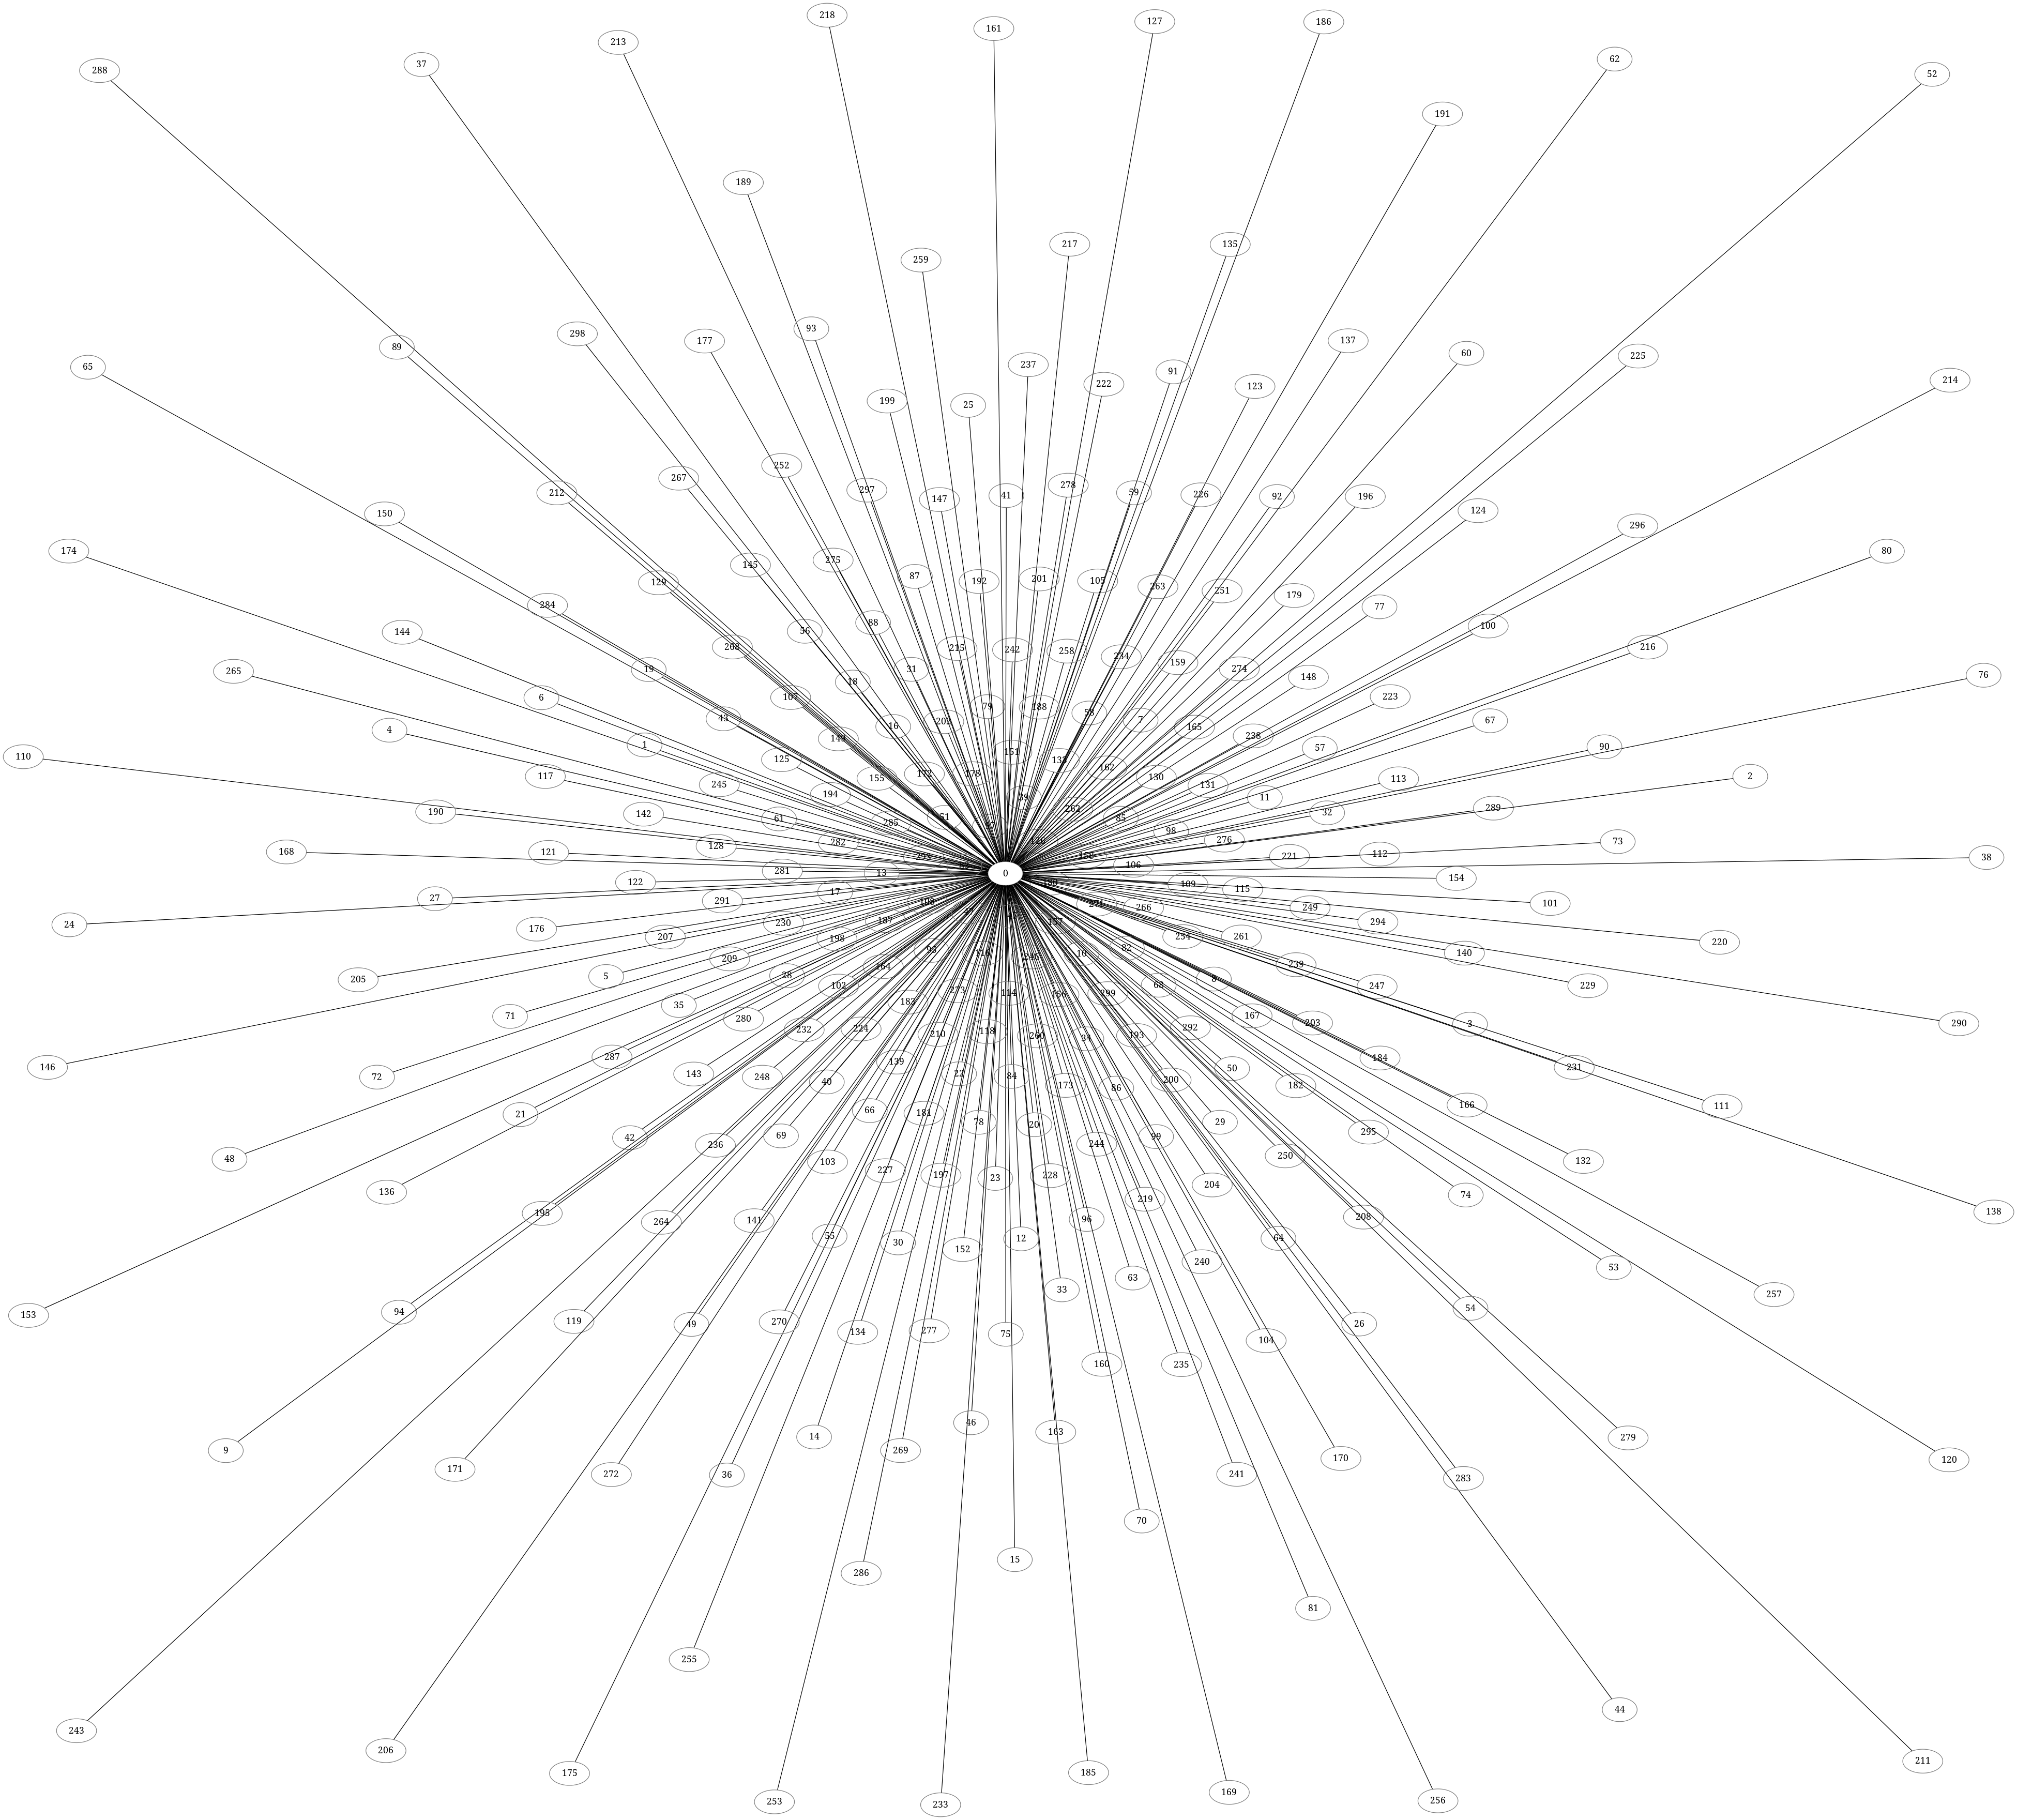
\includegraphics[scale=0.1]{starGraph.png}
  \caption{Example of a Star Graph generated by the Random Graph Algorithm in Figure~\ref{fig:maxM}}
  \label{fig:starGraph}
\end{centering}
\end{figure}

\begin{figure}
\begin{centering}
  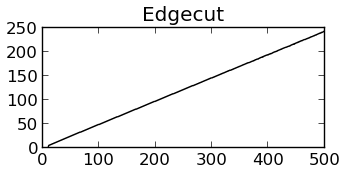
\includegraphics[scale=1]{maxM5-Edgecut.png}
  \caption{This is a graph describing the edgecut of the graphs generated from the parse tree in Figure~\ref{fig:maxM} as a function of the number of vertices in the graph. 
    These results are averaged over 30 random graphs at each size from 0 to 500.}
  \label{fig:maxM-graph}
\end{centering}
\end{figure}

\begin{figure}
\begin{centering}
  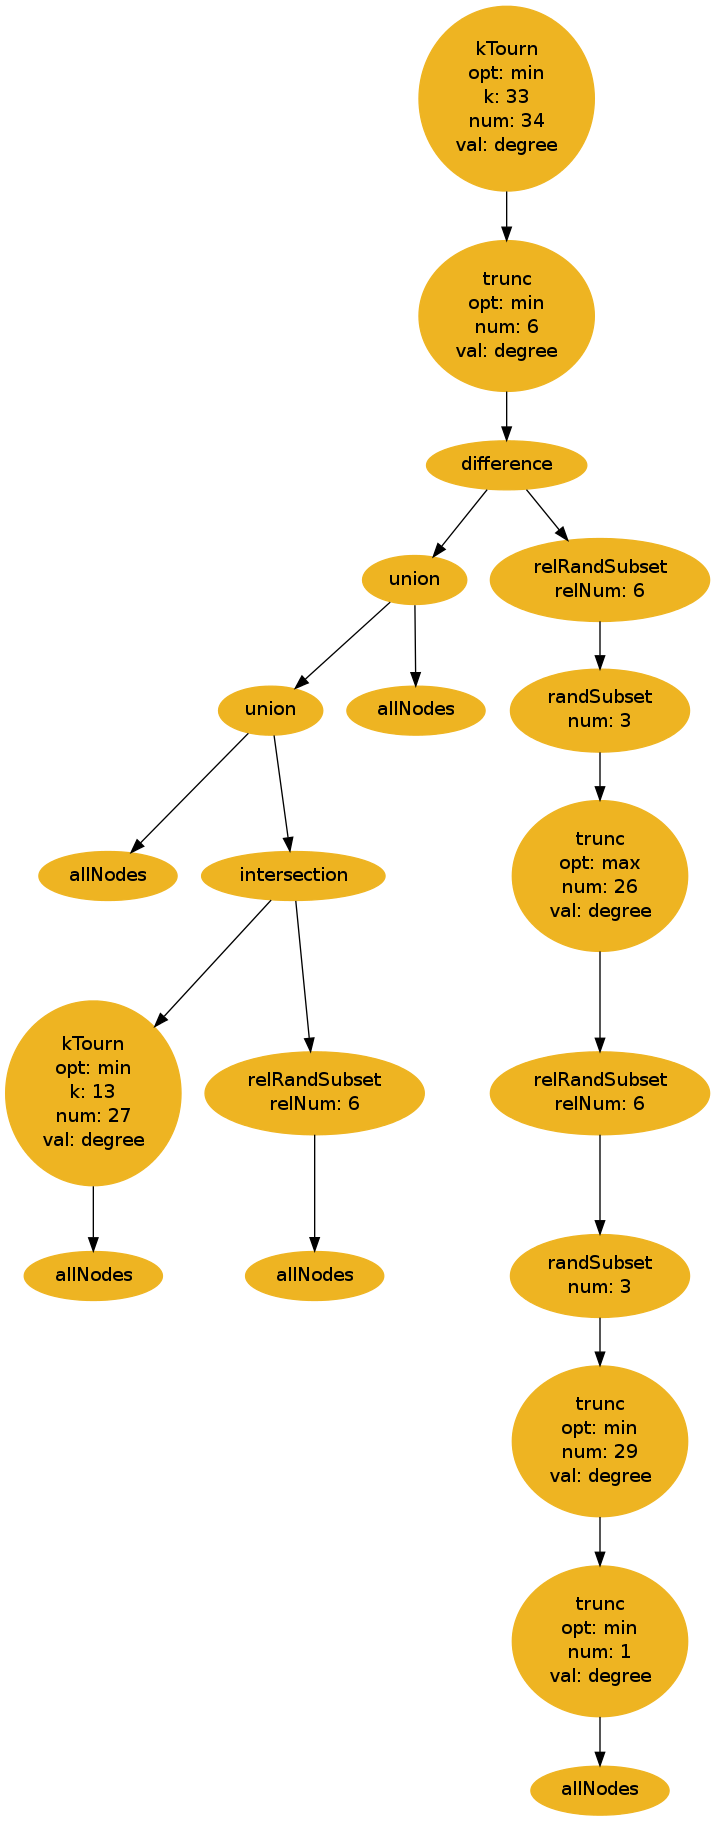
\includegraphics[scale=0.25]{minM.png}
  \caption{Parse Tree of Random Graph Algorithm Found to Minimize the Edgecuts of a Partition and Maximize the Number of Edges}
  \label{fig:minM}
\end{centering}
\end{figure}

\begin{figure}
\begin{centering}
  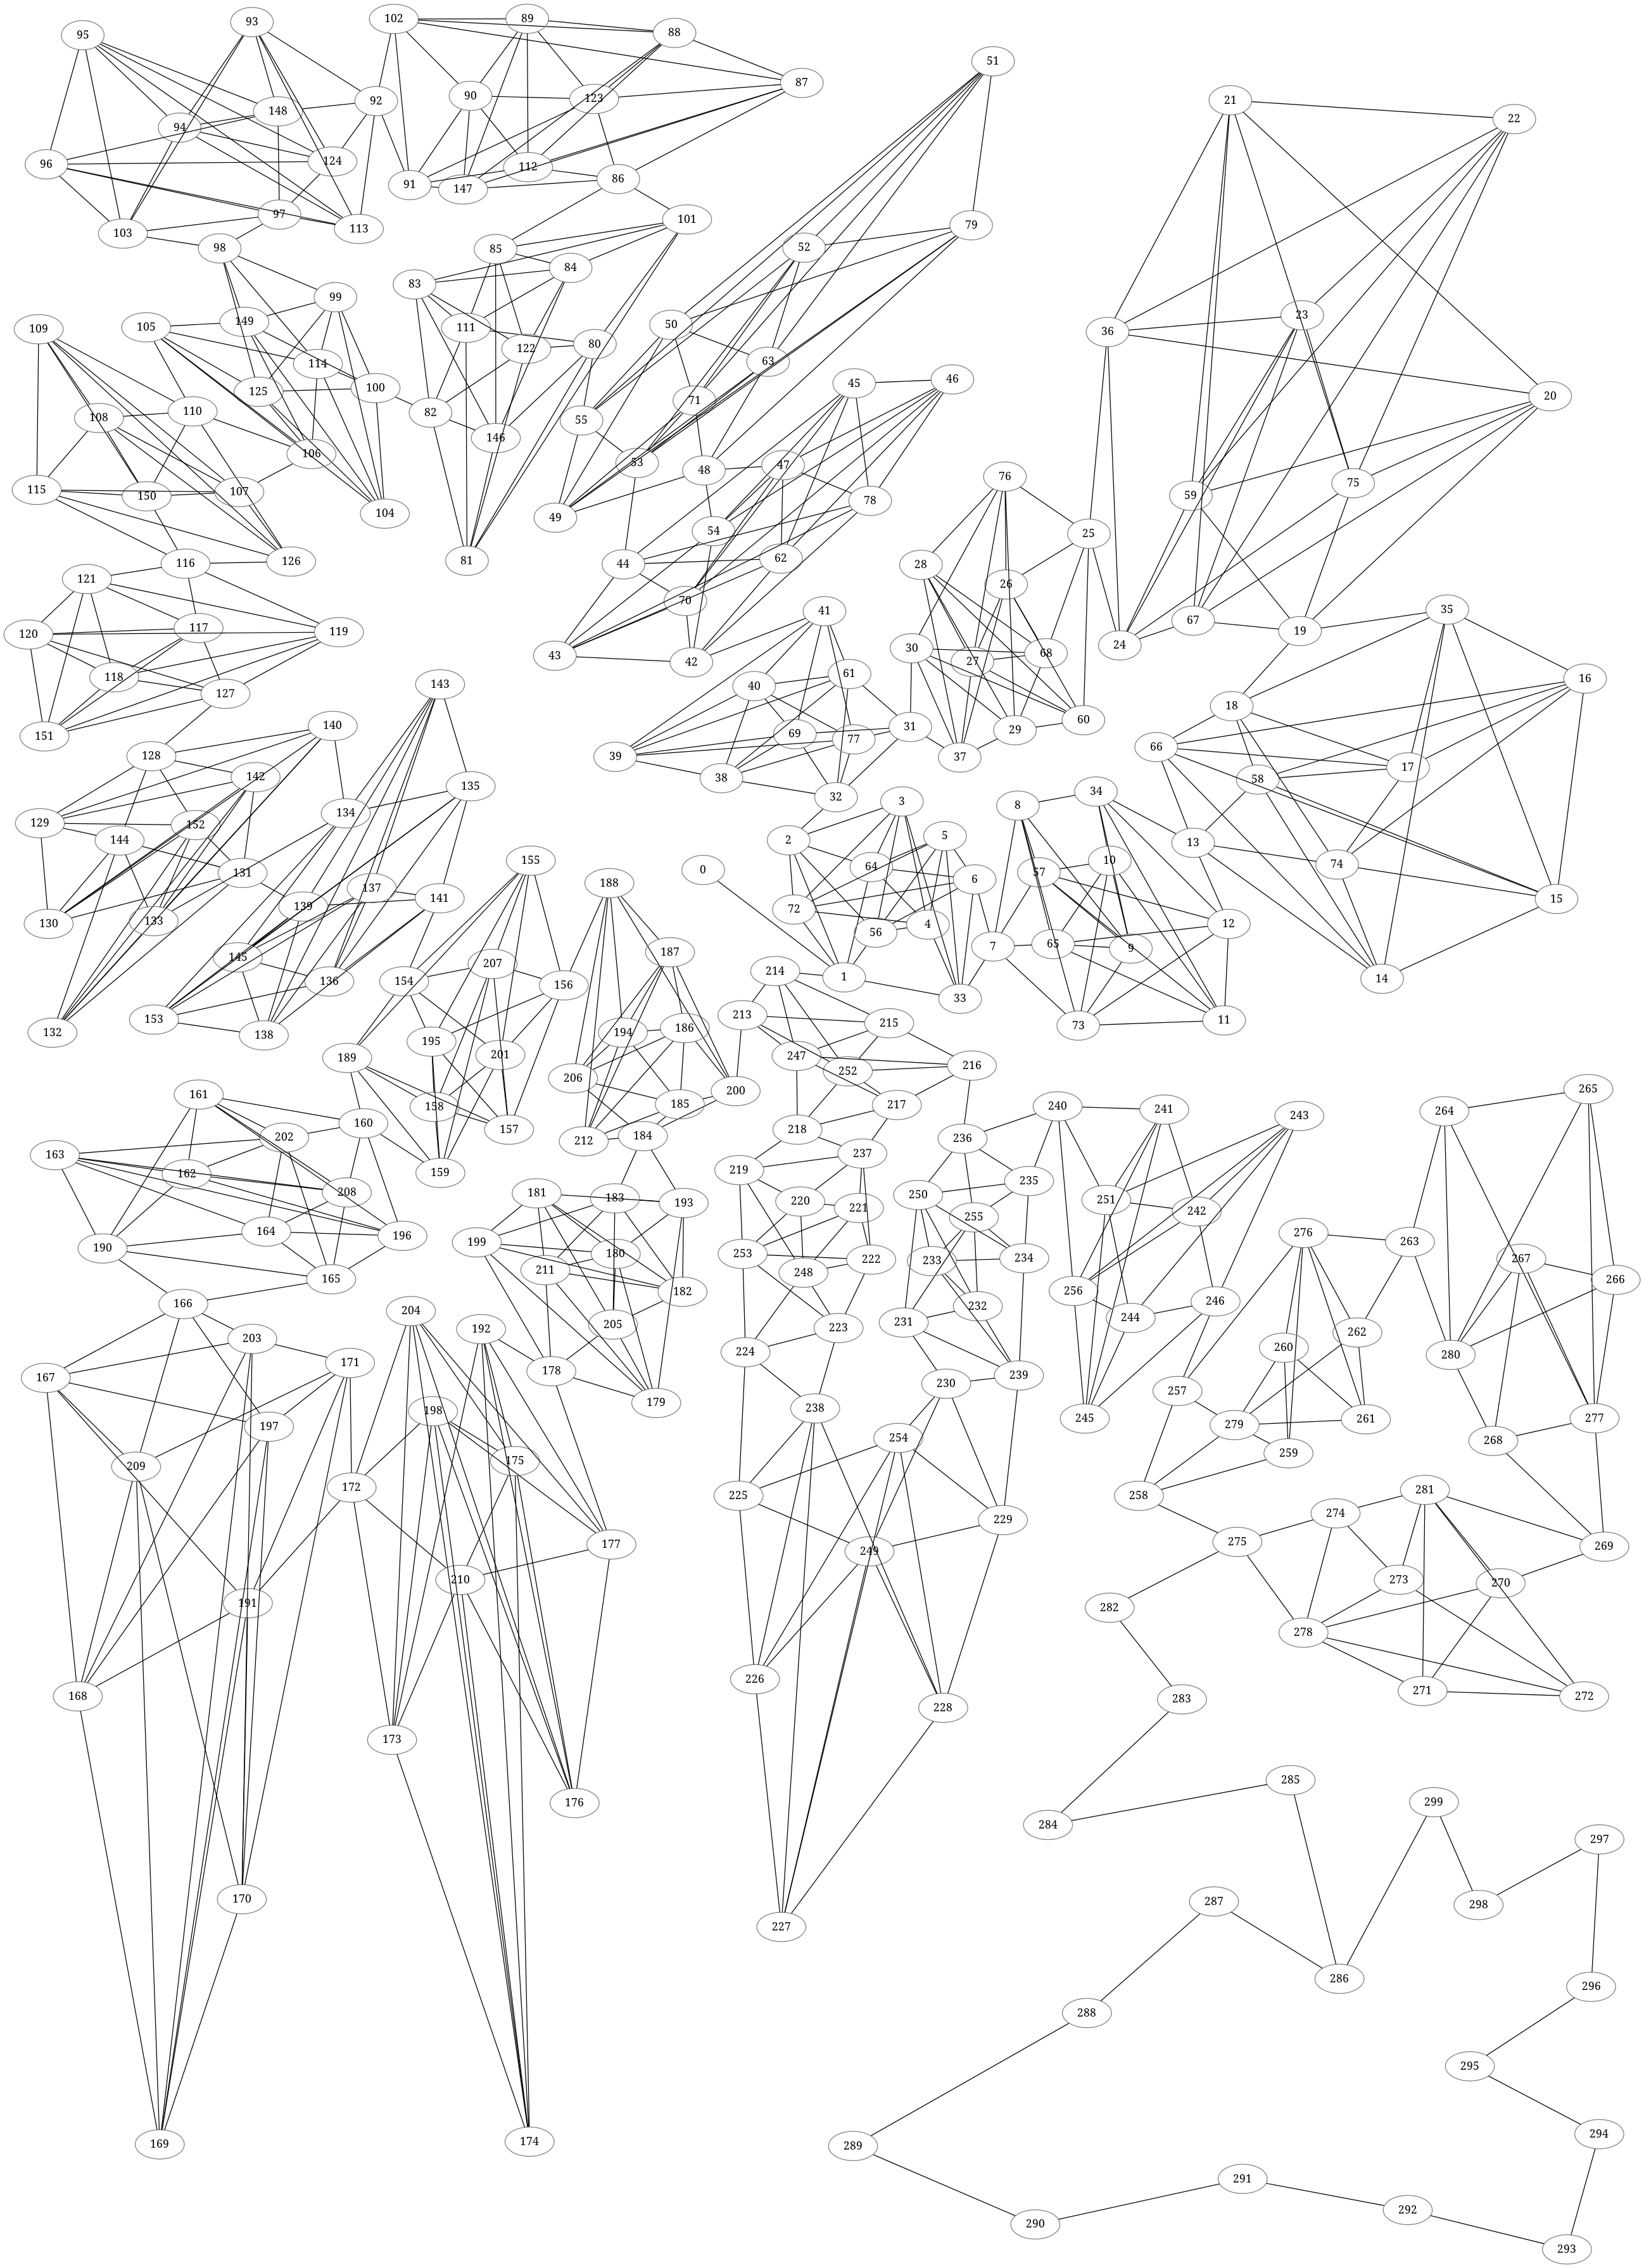
\includegraphics[scale=0.165]{minMGraph.png}
  \caption{Example of a Graph Produced by the Random Graph Algorithm in Figure~\ref{fig:minM}}
  \label{fig:minMGraph}
\end{centering}
\end{figure}

\begin{figure}
\begin{centering}
  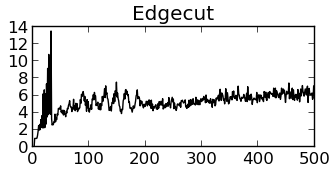
\includegraphics[scale=1]{minM2-Edgecut.png}
  \caption{This is a graph describing the edgecut of the graphs generated from the parse tree in Figure~\ref{fig:minM} as a function of the number of vertices in the graph. 
    These results are averaged over 30 random graphs at each size from 0 to 500.}
  \label{fig:minM-graph}
\end{centering}
\end{figure}


\begin{figure}
\begin{centering}
  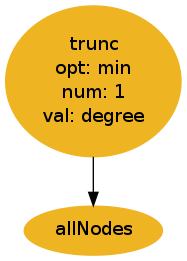
\includegraphics[scale=0.45]{maxE.png}
  \caption{Parse Tree of Random Graph Algorithm Found to Maximize the Average Eccentricity and Minimize the Number of Edges}
  \label{fig:maxE}
\end{centering}
\end{figure}

%\begin{figure}
%\begin{centering}
%  \includegraphics[scale=0.025]{maxEGraph.png}
%  \caption{Example of a Graph Produced by the Random Graph Algorithm in Figure~\ref{fig:maxE}}
%  \label{fig:maxEGraph}
%\end{centering}
%\end{figure}

\begin{figure}
\begin{centering}
  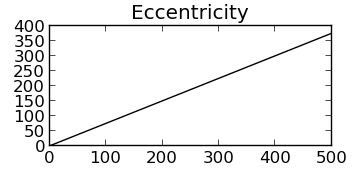
\includegraphics[scale=1]{maxE2-Eccentricity.png}
  \caption{This is a graph describing the average eccentricity of the graphs generated from the parse tree in Figure~\ref{fig:maxE} as a function of the number of vertices in the graph. 
    These results are averaged over 30 random graphs at each size from 0 to 500.}
  \label{fig:maxE-graph}
\end{centering}
\end{figure}


\begin{figure}
\begin{centering}
  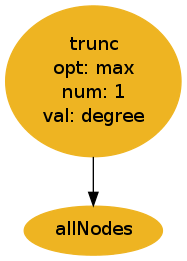
\includegraphics[scale=0.45]{minE.png}
  \caption{Parse Tree of Random Graph Algorithm Found to Minimize the Average Eccentricity and Minimize the Number of Edges}
  \label{fig:minE}
\end{centering}
\end{figure}

\begin{figure}
\begin{centering}
  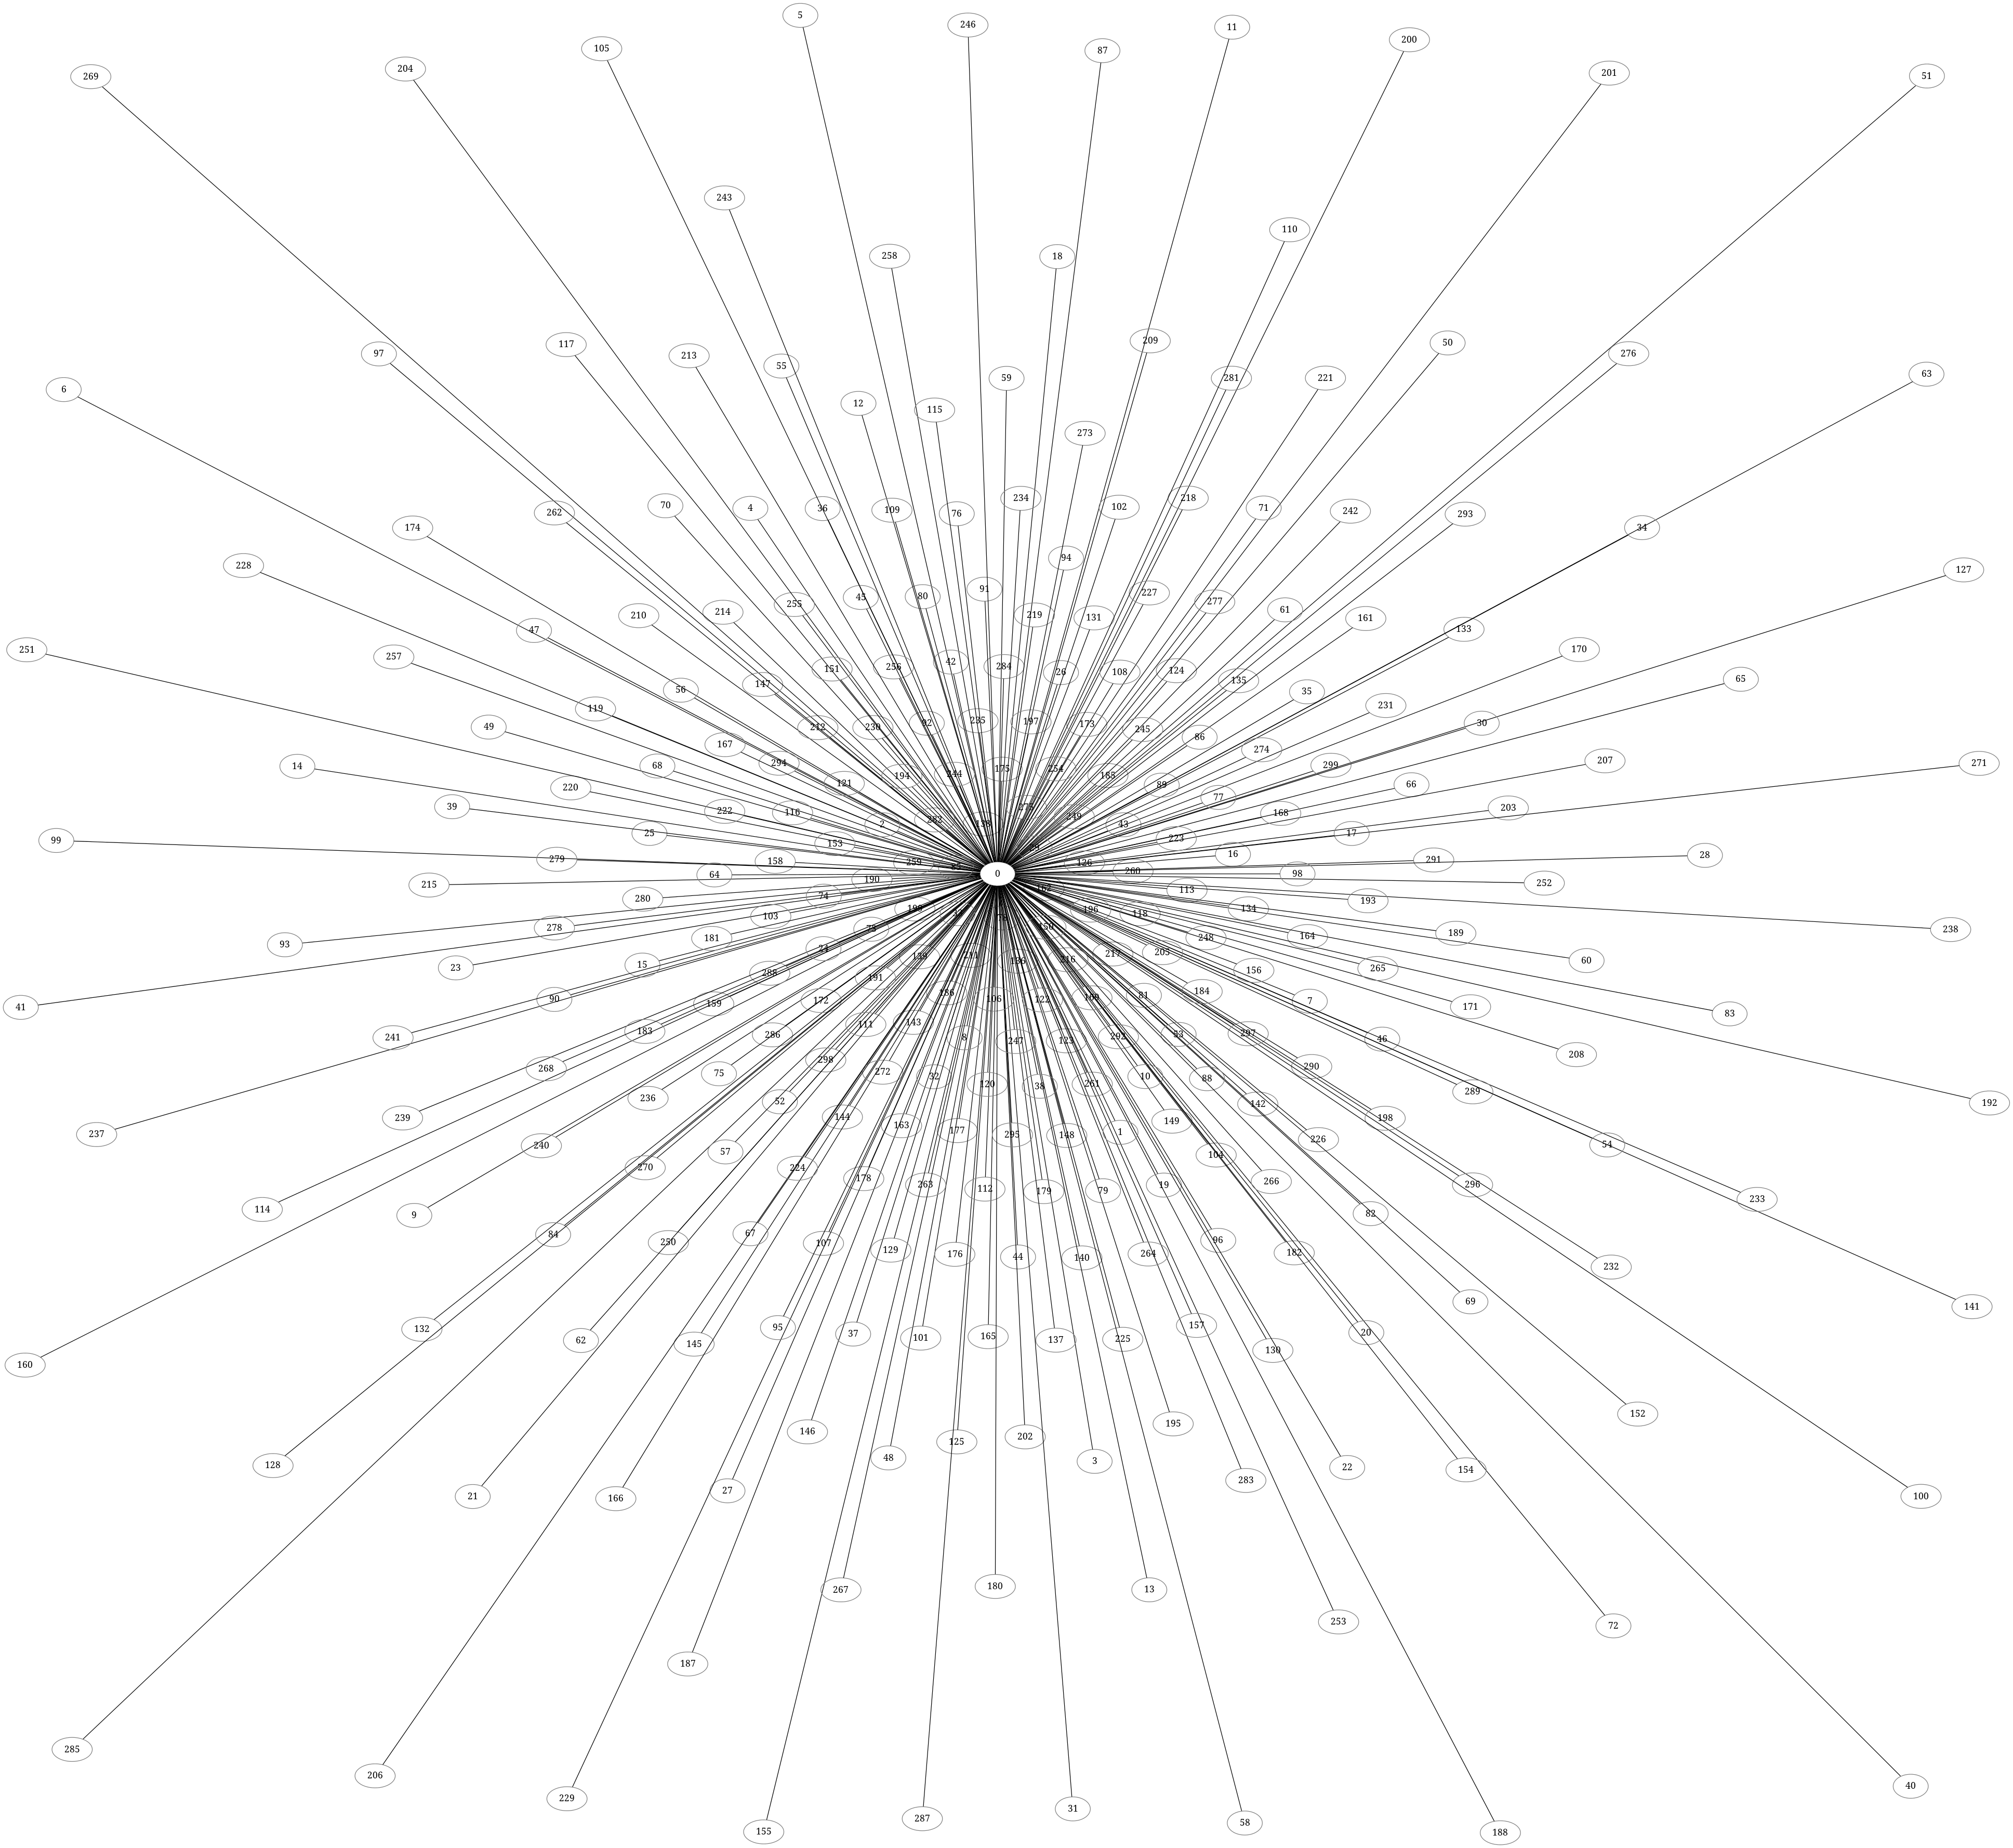
\includegraphics[scale=0.1]{minEGraph.png}
  \caption{Example of a Graph Produced by the Random Graph Algorithm in Figure~\ref{fig:minE}}
  \label{fig:minEGraph}
\end{centering}
\end{figure}

\begin{figure}
\begin{centering}
  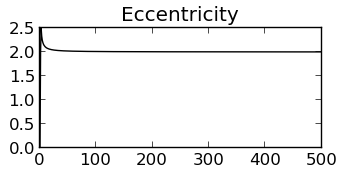
\includegraphics[scale=1]{minE2-Eccentricity.png}
  \caption{This is a graph describing the average eccentricity of the graphs generated from the parse tree in Figure~\ref{fig:maxE} as a function of the number of verticess in the graph. 
    These results are averaged over 30 random graphs at each size from 0 to 500.}
  \label{fig:minE-graph}
\end{centering}
\end{figure}

\section{Discussion}

\subsection{Maximize Partition}
The first experiment was to evolve a Random Graph Algorithm that would generate a graph that would maximize the edge cut of the partition
that the Metis algorithm could find while minimizing the number of edges that were used. The best Random Graph Algorithm that was found
was a Random Graph Algorithm that generated a star graph. The parse-tree representation of this algorithm can be seen in Figure~\ref{fig:maxM}.
An example of the graph produced by this algorithm can be seen in Figure~\ref{fig:starGraph}. This graph is a very good solution to the 
problem of interest. In a star graph there are $n-1$ edges which is the smallest number of edges for a graph to still be connected, and the
partitioning algorithm has to cut $\floor*{\frac{n-1}{2}}$ edges to partition the graph into equal subgraphs. A graph of the edgecut as a function
of the number of vertices can be seen in Figure~\ref{fig:maxM-graph}

\subsection{Minimize Partition}

The second experiment was to evolve a Random Graph Algorithm that would generate a graph that would minimize the edge cut of the partition
that the Metis algorithm could find while maximize the number of edges that were used. The evolved Random Graph Algorithms trained on
this problem had a very distinct structure. They consisted of highly connected structures that were connected by a relatively small number
of edges. This structured allowed the graphs to have a very high edge count while keeping the quality of being partitioned with a small
number of edgecuts. An example of the resulting graph can bee seen in Figure~\ref{fig:minMGraph}. The parse tree representation of the
Random Graph Algorithm which produced this graph can be seen in Figure~\ref{fig:minM}. A graph of the edgecut as a function of the number
of vertices can be seen in Figure~\ref{fig:minM-graph}

\subsection{Maximize Eccentricity}
The third experiment was to evolve a Random Graph Algorithm that would generate a graph that would maximize the average eccentricity of its
vertices while also minimizing the number of edges that were used. The evolved Random Graph Algorithms trained on this problem created
graphs that were a path. The parse-tree representation of this algorithm can be seen in Figure~\ref{fig:maxE}. 
This graph is a very good solution to the problem of interest. A path has an average eccentricity defined by Equation~\ref{eq:Ecc} 
which is the maximum average eccentricity and has $n-1$ edges which is the fewest number of edges possible 
in a connected graph.

\begin{equation}
\label{eq:Ecc}
Average~Eccentricity = \frac{n(n-1) - \frac{\ceil*{\frac{n}{2}}(\ceil*{\frac{n}{2}}-1)}{2} - \frac{\floor*{\frac{n}{2}}(\floor*{\frac{n}{2}}-1)}{2}}{n}
\end{equation}

In the above equation $n$ is the number of vertices in the graph. A graph of this function can be seen in Figure~\ref{fig:maxE-graph}.

\subsection{Minimize Eccentricity}
The fourth experiment was to evolve a Random Graph Algorithm that would generate a graph that would minimize the average eccentricity of
its vertices while minimizing the number of edges that were used. The evolved Random Graph Algorithms trained on this problem created star
graphs. The parse-tree representation of this algorithm can be seen in Figure~\ref{fig:minE}. This graph is a good solution to the problem.
A star graph has an average eccentricity of $\frac{2n-1}{n}$ and has only $n-1$ edges. The only graphs with a smaller average eccentricity
would have many more vertices and therefore wouldn't be minimizing the number of edges. An example of the resulting graph can be seen in Figure~\ref{fig:minEGraph}.
A graph of the average eccentricity as a function of the number of vertices can be seen in Figure~\ref{fig:minE-graph}. 

\subsection{Observations}


\begin{figure}
\begin{centering}
  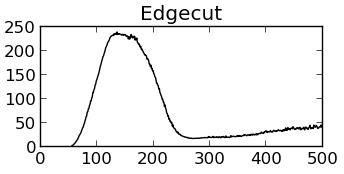
\includegraphics[scale=1]{mislead.png}
  \caption{This is a graph describing the edgecut of the partition of the graphs generated from a parse-tree that attempted to minimize the edgecut as a function of the number of vertices in the graph. 
    These results are averaged over 30 random graphs at each size from 0 to 500.}
  \label{fig:mislead}
\end{centering}
\end{figure}



It was discovered that the evaluation method that was implemented has the ability to be misleading about the true nature of how the
Random Graph Algorithm performs. Figure~\ref{fig:mislead} shows the edgecut of partition of graphs generated from one of the parse-trees
that was traind to minimize the edgecut. As can be seen in the figure, if a graph was generated of size 100-200 that the edgecut would be
much higher than would be expected based on the results during evolution. This demonstrates a flaw in the evaluation of the Random Graph Algorithms.
An improvement to the current method would be to sample periodically up until the maximum graph size to ensure that the trend of the
properties of interest would be known regardless of size of the graph.



\section{Conclusion}
This paper proposed a GP method to evolve Random Graph Algorithms that would create graphs that have a user specified property. As demonstrated
in the experiments, the GP was able to create Random Graph Algorithms which satisfied the criteria defined by the fitness functions shown. While thes
fitness functions were simple, the results demonstrate that this method can sucessfully create Random Graph Algorithms that have the user-defined 
properties of interest. 

It was discovered that while the evaluation method for assigning a fitness to the Random Graph Algorithms is efficient, it does not however provide
enough evolutionary pressure to ensure that the properties can be found at an arbitrary point during generation. The current evaluation method only 
provides the probabilistic certainty that the properties of interest exist in the random graphs at the size that they were evolved. A more complex evaluation
method needs to be constructed to gauge the presence of the desired properties at intermittent times during the creating of the random graph. This will
help insure that the properties that are desired exist in all graphs generated regardless of size. 


\section{Future Work}
The first addition that needs to be made to the proposed method is the improved fitness evaluation. This will allow for the GP to create Random Graph
Algorithms that will be more consistent. The produced Random Graph Algorithms will have a higher likelihood of having the desired properties at
graph sizes larger and smaller than the size they were evolved on.

Another proposed addition to this method is adding the capability to evolve Random Directed Graph Algorithms. This will add more applications
that this method could be applied to. One such application is the generation of control flow graphs that simulate program control flow graphs. Extracting
control flow graphs from programs is a difficult task and is not very accurate. By creating a Random Directed Graph Algorithm to generate control flow graphs,
this would give algorithm developers a much larger data set to develop their algorithms on. 


\bibliographystyle{abbrv}
\bibliography{sigproc} 


\end{document}


